%\chapter{Optimizaci\'on de la representaci\'on de datos}

% Approximate nearest neighbors by  deep  hashing on large-scale search: Comparison of representations and retrieval performance 
\chapter{Búsqueda aproximada vía \textit{Deep Hashing}}

\section{Consideraciones Iniciales}
 
\versal{L}a disponibilidad cada vez mayor de datos en diversos dominios ha creado la necesidad de desarrollar técnicas y métodos para descubrir el conocimiento a partir de volúmenes masivos de datos, motivando muchos trabajos de investigación en bases de datos, \textit{machine learning} y comunidades de recuperación de información. Esto ha impulsado el desarrollo de técnicas escalables y eficientes para organizar y recuperar este tipo de datos. \textit{Similarity search} ha sido el enfoque tradicional para la recuperación de información. Aunque se han propuesto varios algoritmos de búsqueda de similitud para acelerar las consultas de similitud, la mayoría de ellos se ven afectados por la maldición de la alta dimensionalidad de los datos. Recuperar datos complejos causa problemas de estabilidad cuando la dimensionalidad de los datos es muy alta \cite{aleman_high_dimensional}.


Se han estudiado diferentes enfoques para resolver el problema de de la alta dimensionalidad de los datos. Una de las líneas de investigación es relajar la precisión de la consulta para acelerar el tiempo de consulta. Potencialmente, este enfoque es factible para aplicaciones que no requieren respuestas exactas y cuya velocidad es más importante que la precisión de búsqueda. Además, la definición del espacio métrico ya conduce a una aproximación de la respuesta verdadera, y por lo tanto una segunda aproximación en el tiempo de búsqueda puede ser aceptable \cite{cit:avez99searching}.

Se propusieron algoritmos de kNN aproximados basados en \textit{hashing} para consultar conjuntos de datos de alta dimensión debido a su alta velocidad de recuperación y bajo costo de almacenamiento. \acf{LSH} \cite{lsh} es una de las recientes técnicas basadas en $hash$ propuestas para organizar y consultar datos de alta dimensión. De hecho, LSH es una de las pocas técnicas que proporciona análisis teóricos sólidos y pérdida predecible de precisión en los resultados. Sin embargo, existe una dependencia en los valores de los parámetros para los esquemas de búsqueda de similitud aproximada basados en LSH, que determinan el número de funciones hash y el número de tablas hash.

Para responder consultas de similitud, \ac{LSH} busca solo regiones, que están representadas por \textit{buckets}, a los que se aplica el hash del objeto de consulta (es decir, los candidatos de los \textit{buckets}  que contienen los objetos del conjunto de datos con una alta probabilidad de similitud con el objeto de consulta). Por lo tanto, no es necesario explorar completamente los datos de índice, y solo los objetos en los candidatos de los \textit{buckets}  que requieren un procesamiento adicional de acuerdo con la condición de consulta (por ejemplo, $ d(x,q) \leq r $) \cite{DBLP:journals/jidm/OcsaS10}.

Los métodos de $hashing$ producen una representación compacta  para realizar   tareas de clasificación usando \textit{hash-codes}. Cuando el proceso es supervisado, los códigos $hash$ se entrenan usando etiquetas ($labels$) en los datos de entrenamiento. Inspirado por los avances recientes en \acf{CNN} \cite{ImageNet}, muchos métodos mejoran la precisión de la recuperación de similitud al usar CNN como extractor de características y luego crean un código $hash$ compacto. En un trabajo reciente \cite{kLin:DH}, un método de hashing supervisado entrena el modelo con una capa oculta de tipo \textit{binary-hash} como características para tareas de clasificación de imágenes. Al combinar la extracción de características de imagen y el aprendizaje de códigos binarios, estos métodos han demostrado una alta precisión. Sin embargo, existe un compromiso entre el error de clasificación y el error de cuantificación: las activaciones de las capas inferiores son más comunes \cite{DBLP:journals/corr/YosinskiCBL14}, por lo que el entrenamiento es más efectivo. Sin embargo, las capas inferiores tienen mapas de activación más grandes (muchos nodos), que son más difíciles de codificar lo que lleva a un compromiso.


\subsection{Approximate Nearest Neighbors \& Deep Hashing}

\subsubsection{Hashing para la Búsqueda del Vecino más Cercano}

El problema del vecino más cercano, busca el punto más cercano en un conjunto de datos para un punto de consulta específico y es importante en muchas áreas de Ciencia de la Computación. La figura \ref{searchmodelcap5} ilustra el modelo de búsqueda de similitud para la búsqueda ANN utilizando hashing. Cada objeto del conjunto de datos se comprime utilizando códigos $hash$ que generan el nuevo espacio de búsqueda en el espacio reducido. Por lo general, se usa un índice para organizar el conjunto de datos de manera que los objetos cercanos en el espacio original estén juntos bajo cierta probabilidad en el espacio reducido. En el momento de la consulta, el objeto de consulta se asigna a regiones con alta probabilidad de encontrar objetos similares. Finalmente, las regiones de calificación se analizan para informar solo los objetos que satisfacen la condición de consulta.
\begin{figure}[htp]
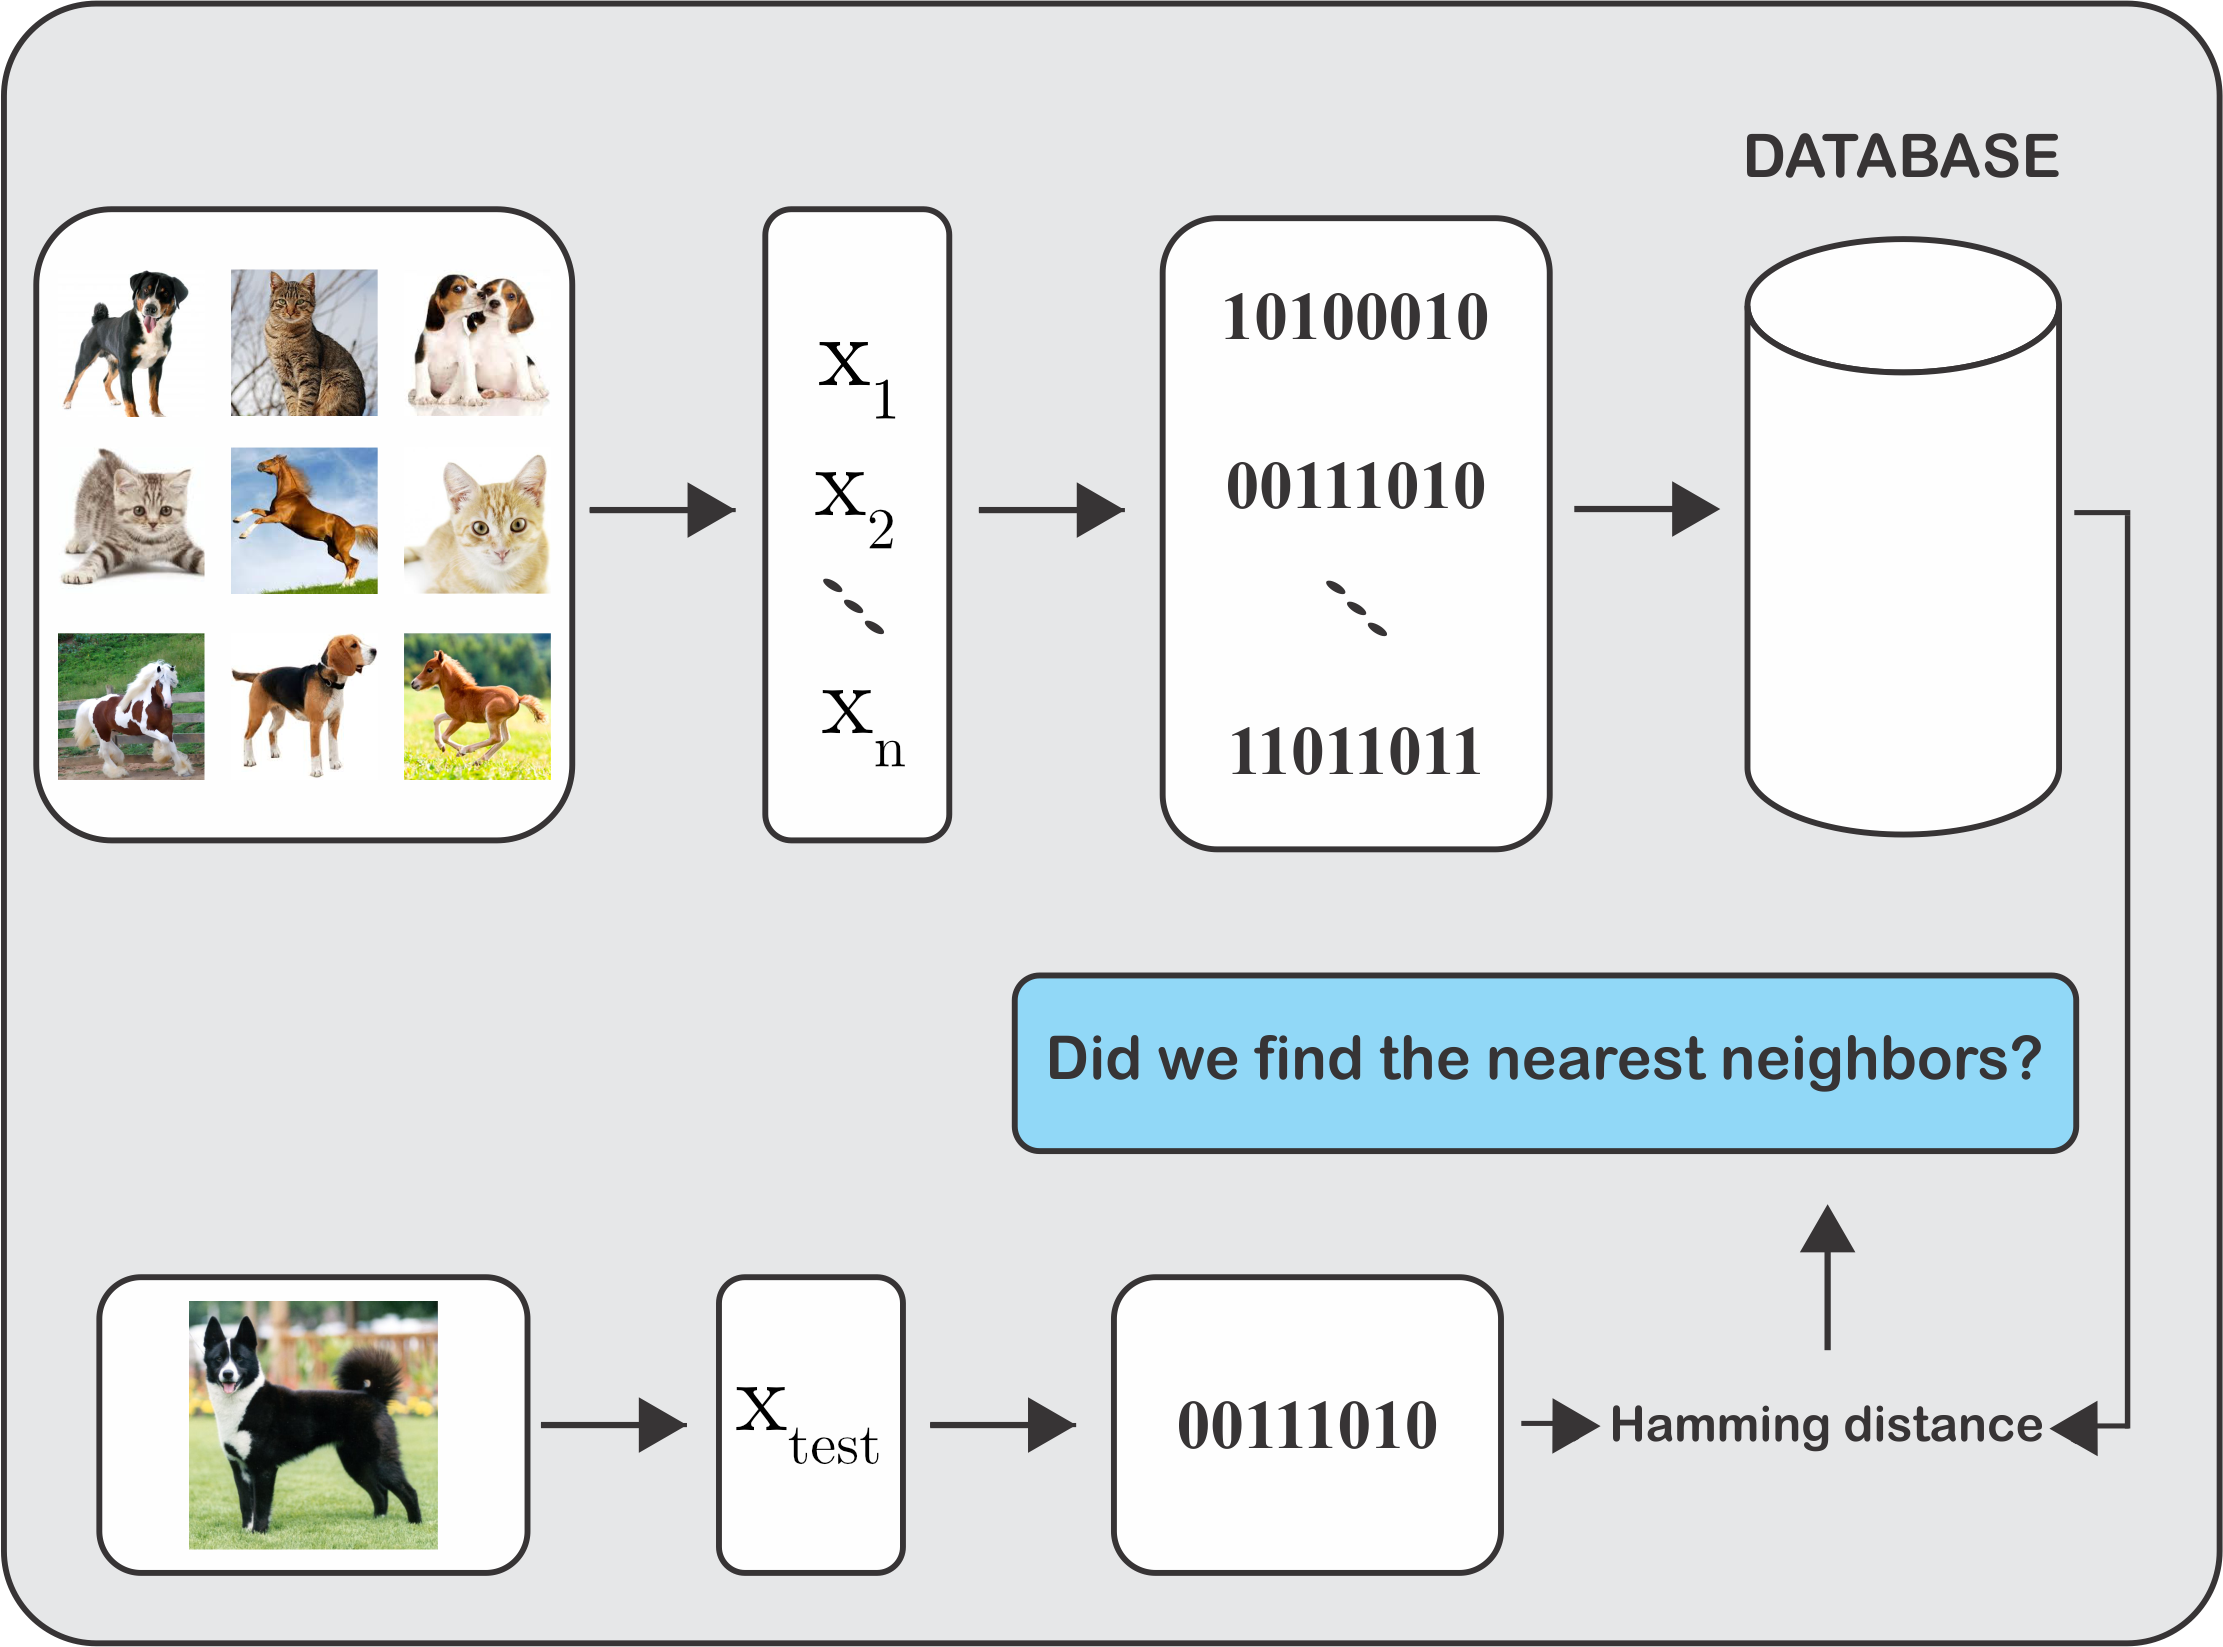
\includegraphics[width=0.7\columnwidth]{chapter5/ima1.png}
\centering
\caption{ Hashing para la búsqueda del vecino más cercano. Comprimir un conjunto de vectores  $(x_i)^{n}_{i=1}, x_i \in \mathbf{R}^d $ }
\label{searchmodelcap5}
\end{figure}

\subsubsection{Supervised Hashing}
La figura \ref{supervisedhashingcap5} ilustra un modelo de búsqueda de similitud para Hashing supervisado. Cada objeto del conjunto de datos se comprime utilizando códigos $has$h que generan el nuevo espacio de búsqueda en el espacio reducido. Cuando el proceso es supervisado, los códigos se entrenan usando etiquetas ($labels$) en los datos de entrenamiento.
\begin{figure}[htp]
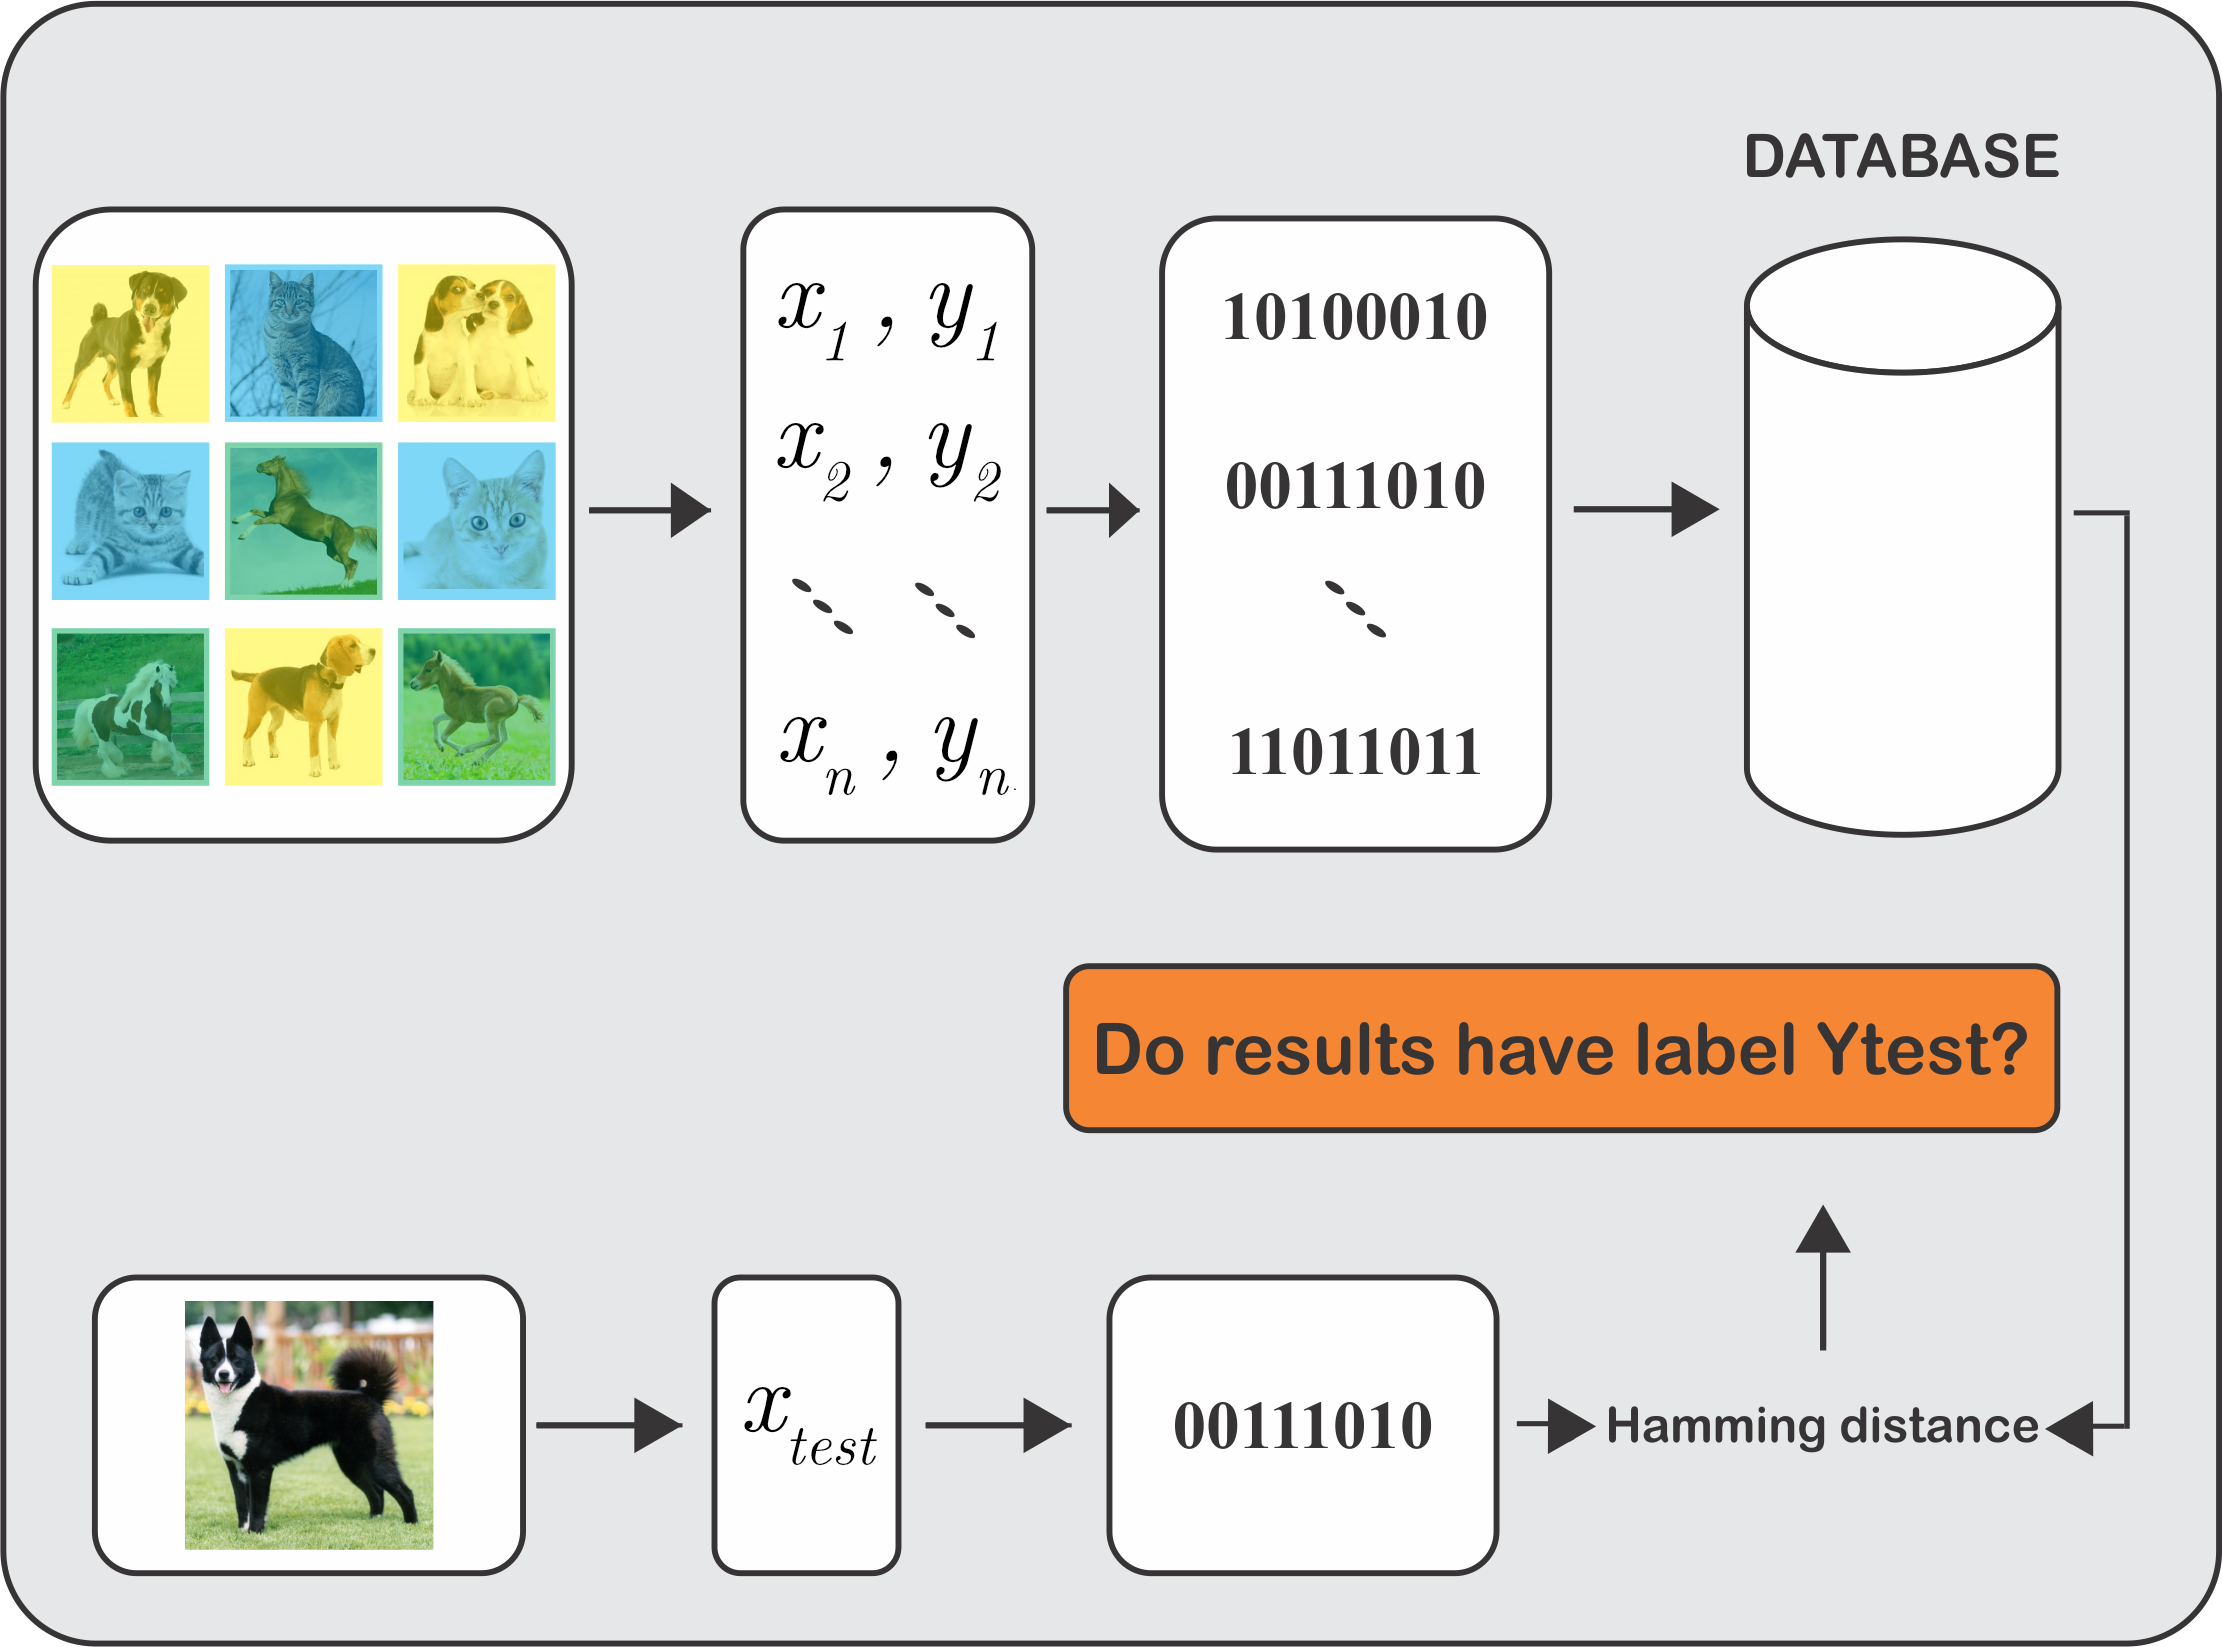
\includegraphics[width=0.7\columnwidth]{chapter5/ima2.png}
\centering
\caption{ Supervised Hashing: comprime un conjunto de vectores y sus etiquetas $((x_i,y_2))^{n}_{i=1}, x_1\in \mathbb{R}^{d}, y_1 \in \{1,...,L\} $.}
\label{supervisedhashingcap5}
\end{figure}

\begin{description}
\item [Supervised Hashing (SH)] : etiquetas $ y_i $ asociados a todos los puntos $ x_i (i = 1, ..., n) $ en el conjunto de datis
\item [Semi-supervised hashing (SSH)] : etiquetas $ y $ asociados solo a  $ n_{label} $ muestras
\end{description}

\subsection{Protocolos de evaluación de recuperación}

En esta sección, describimos los protocolos utilizados en la literatura para SSH y SH y explicamos cómo una estrategia simple resuelve eficientemente los problemas similares.

\subsubsection{Protocolos de evaluación de SH y SSH}

SSH consiste en indexar un conjunto de datos de $ n $ imagenes $ \mathcal{I}_{train} $, de los cuales un subconjunto $ \mathcal{I}_{label} \subseteq \mathcal{I}_{train} $ es etiquetado. Pero, SH es el caso extremo $ \mathcal{I}_{label} = \mathcal{I}_{train} $. Si tenemos una imagen de consulta sin etiqueta $ q $, el sistema debe devolver una lista ordenada de imágenes de $ \mathcal{I}_{train} $. Para evaluar, tenemos un conjunto de datos de consultas; el evaluador conoce todas las etiquetas de las consultas, así como las etiquetas en $ \mathcal{I}_{train} $. El rendimiento se mide por precisión o \textit{mean average precision} (mAP).

Entonces, dada una consulta $ q $, si la imagen $ i^{th} $ es correcta para $ q $ definimos $ \delta(q, i) = 1 $, y $ 0 $ de lo contrario. La precisión en el rango $ k $ para kNN viene dada por $ P(q, k) = \tfrac{1}{k} {\sum}_{i = 1}^{k} \delta(q, i) $. Denotando por $ cl(q) = {\sum}_{i = 1}^{n} \delta(q, i) $ el número total de imágenes correctas en $ \mathcal{I}_{train} $, y la precisión promedio en $ k $ es $ AP(q, k) = \tfrac{1}{cl(q)} {\sum}_{i = 1}^{k} \delta(q, i) P( q, i) $. El mAP en $ k $ (o simplemente mAP cuando $ k = n $) es el AP promedio sobre todas las consultas de prueba \cite{sablayrolles2016should}.

\subsubsection{Representación de datos y medidas de similitud}\label{sec:methods_reduce}

Se han propuesto muchos métodos en la bibliografía para representar datos complejos con dimensionalidades reducidas, que admiten búsquedas de similitud y tareas de minería de datos. Estos métodos se pueden representar en dos categorías: representaciones de datos adaptativos y representaciones de datos no adaptativos \cite{wang13}.

En la representación de  tipo adaptativo   tenemos los siguientes métodos: \textit{Singular Value Decomposition} (SVD) que transforma la serie de tiempo $ A_i $ en otra serie de tiempo $ B_i $ de longitud $ n $ cuyos elementos están en orden decreciente \cite{Bettaiah14}. \textit{Principal Component Analysis} (PCA) que involucra procedimientos matemáticos que transforman un número de (posibles) variables de correlación en un número (más pequeño) de variables no correlacionadas, llamadas componentes principales \cite{wekwek}. En PCA, los datos se resumen como una combinación lineal de conjuntos de vectores ortonormales. La PCA actúa de forma similar a los Autoencoders (AE) que aplican la retropropagación estableciendo los valores objetivo para que sean iguales a las entradas $ y(i) = x(i) $ \cite{wekwek}.

Los métodos más comunes utilizados en la representación de datos no adaptativos son: \textit{Discrete Cosine Transformation} (DCT), es una transformación ortonormal real. DCT es similar a \textit{discrete Fourier transform} (DFT) \cite{Faloutsos94}, con la diferencia de que usa funciones de coseno en lugar de senos y cosenos para transformar del dominio de tiempo al dominio de frecuencia \cite{Bettaiah14}. \textit{Discrete Wavelet Transformation} (DWT) procesa datos a diferentes escalas o resoluciones en contraste con DFT \cite{Faloutsos94} donde solo los componentes de frecuencia se consideran  \cite{Bettaiah14}.

Junto con esto, hay más de una docena de medidas de distancia para la búsqueda de similitudes en la literatura. Las medidas de similitud más comunes utilizadas son Euclidean, Manhattan y Minkowski. La distancia euclidiana y la de Manhattan satisfacen algunas propiedades matemáticas: no negatividad, identidad de indiscernibles, simetría, desigualdad de triángulo \cite{han2011data}.

\subsection{Dimensión fractal y reducción de dimensionalidad}

Como se mostró \cite{citeulike:fractal:encoders}   un buen algoritmo de reducción de dimensionalidad   proyecta los datos en un espacio de características con dimensión cercana a la dimensión fractal (FD) de los datos en el espacio original y conserva las propiedades topológicas.

Por lo tanto, para encontrar la dimensión objetivo ($ m $), podemos seguir la siguiente heurística. Podemos comenzar con el valor en $ m_1 = 2^2 $, calcular el FD del nuevo espacio con solo eso, luego incrementar el valor en $ m_2 = 2^3 $, recalcular el FD, y continuar haciendo esto hasta que $ t(m_t = 2^t) $ donde podemos ver un aplanamiento en la dimensión fractal, lo que significa que más características no cambian la dimensión fractal del conjunto de datos.
 
\subsection{Comparación de representaciones de datos}
\subsubsection{Dimensión fractal y reducción de dimensionalidad}\label{sec:fractal-dimension}

Para obtener la representación más general para el aprendizaje, algunos autores sugieren utilizar la salida de la última capa convolucional de la CNN \cite{DBLP:journals/corr/SablayrollesDJU16}. En esta investigación, usamos esta capa  para la extracción de características. Sin embargo, el espacio reducido donde viven estos datos tienen mucha densidad (muchos nodos en la capa convolucional). El objetivo de esta sección es análizar los métodos de reducción de dimensionalidad y buscar un espacio  donde puedan existir estos datos sin perder información.
\begin{figure}[htbp]
\centering
\subfigure[Conjunto de datos MNIST]{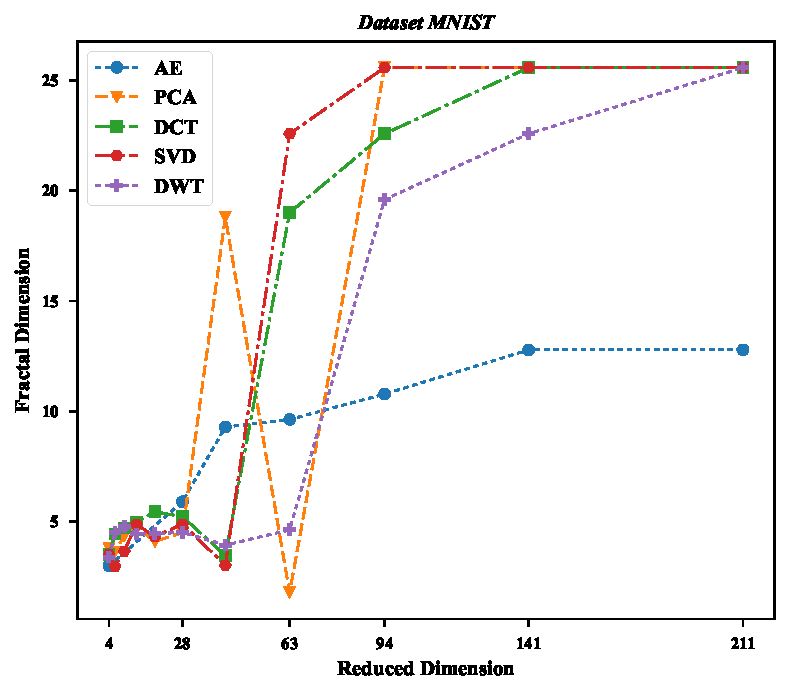
\includegraphics[width=70mm]{chapter5/fig-MNIST.pdf}}
\subfigure[Conjunto de datos CIFAR-10]{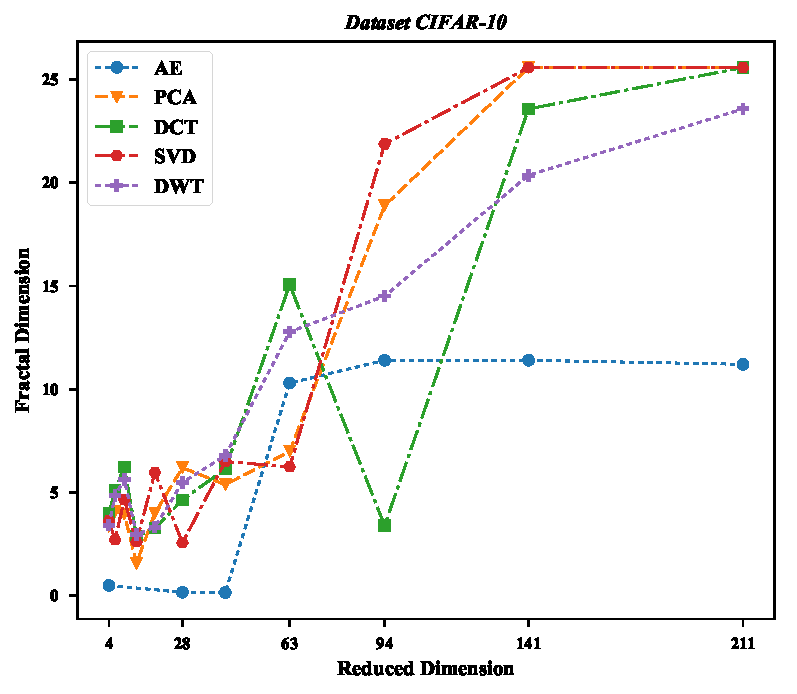
\includegraphics[width=70mm]{chapter5/fig-CIFAR10.pdf}}
\subfigure[Conjunto de datos SVHN]{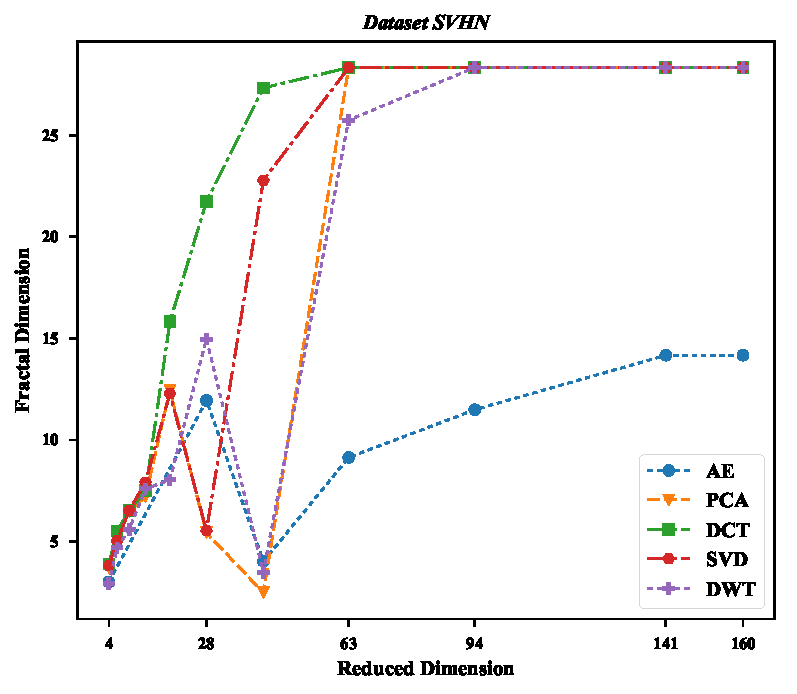
\includegraphics[width=70mm]{chapter5/fig-SVHN.pdf}}
\subfigure[Conjunto de datos AGNEWS]{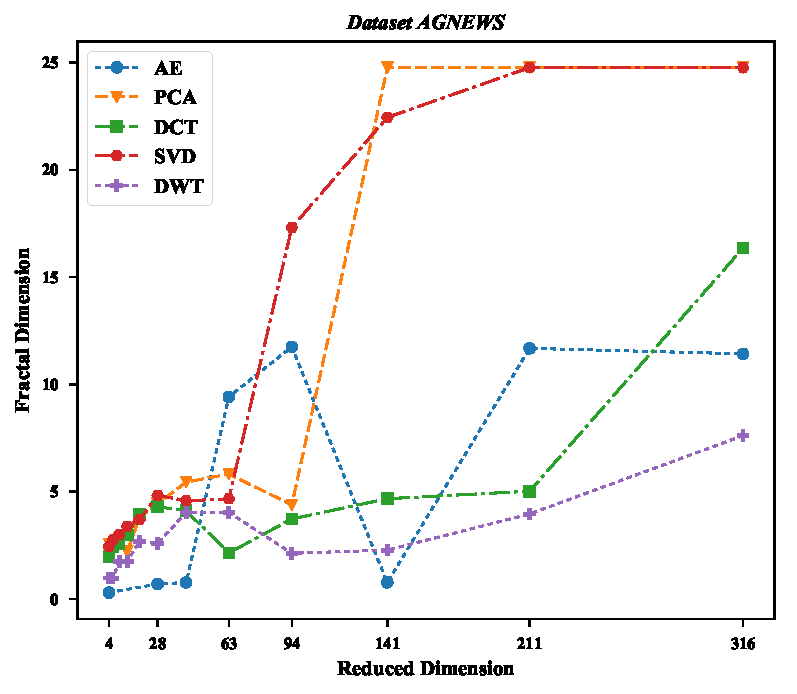
\includegraphics[width=70mm]{chapter5/fig-AGNEWS.pdf}}
\caption{Dimensiones Fractal para diferentes métodos de reducción.} \label{fig:datasetscap5}
\end{figure}


Hemos implementado los métodos de reducción descritos en la sección \ref{sec:methods_reduce}, y los aplicamos en los vectores característicos de los conjuntos de datos MNIST \cite{lecun-mnisthandwrittendigit-2010}, CIFAR-10 \cite{cifar10}, SVHN \cite{svhn} y AgNews \cite{DelCorso:2005:RSN:1060745.1060764}. Para nuestros experimentos, estos vectores de características serán los datos de entrada, y utilizaremos la dimensión fractal para medir su grado de representación.

Podemos analizar el comportamiento de la dimensión Fractal usando diferentes métodos de reducción usando las figuras \ref{fig:datasetscap5}. Con la ayuda de estos gráficos, se puede visualizar  que las curvas generadas se estabilizan a medida que aumenta la dimensión reducida, de acuerdo con los experimentos realizados podemos proponer la siguiente hipótesis: "La aproximación de la dimensión reducida óptima es el valor inicial donde la curva del dimensión fractal vs. la dimensión reducida se estabiliza ". Entonces, cualquier reducción de dimensión después del punto de estabilidad, no reducirá la pérdida de información. Para demostrar esto, evaluamos la precisión de clasificación de las dimensiones reducidas, generadas por los métodos PCA y Autoencoders. El método de clasificación que vamos a utilizar será la clasificación KNN. Los resultados se muestran en la tabla \ref{table-result}.

\begin{table}[]
\centering
\caption{Precisión (P) de la clasificación usando el clasificador KNN  en los conjuntos de datos  MNIST, CIFAR-10, SVHN y Agnews  utilizando  AutoEncoders y PCA como métodos de reducción de dimensionalidad.}
\label{table-result}
\begin{tabular}{c|cc|cccc|}
\cline{2-7}
\multicolumn{1}{l|}{}                           & \multicolumn{2}{c|}{ORIGINAL}                                               & \multicolumn{2}{c|}{AE}                                                       & \multicolumn{2}{c|}{PCA}                                  \\ \cline{2-7} 
\multicolumn{1}{l|}{}                           & \multicolumn{1}{c|}{\cellcolor[HTML]{E6E6E6}Dim.} & P                    & \multicolumn{1}{c|}{\cellcolor[HTML]{E6E6E6}Dim.} & \multicolumn{1}{c|}{P} & \multicolumn{1}{c|}{\cellcolor[HTML]{E6E6E6}Dim.} & P  \\ \hline
\multicolumn{1}{|c|}{}                          & \cellcolor[HTML]{E6E6E6}                          &                         & \cellcolor[HTML]{E6E6E6}63                        & 0.980                     & \cellcolor[HTML]{E6E6E6}42                        & 0.981 \\
\multicolumn{1}{|c|}{}                          & \cellcolor[HTML]{E6E6E6}                          &                         & \cellcolor[HTML]{E6E6E6}141                       & 0.982                     & \cellcolor[HTML]{E6E6E6}94                        & 0.979 \\
\multicolumn{1}{|c|}{\multirow{-3}{*}{MNIST}}   & \multirow{-3}{*}{\cellcolor[HTML]{E6E6E6}800}     & \multirow{-3}{*}{0.982} & \cellcolor[HTML]{E6E6E6}316                       & 0.982                     & \cellcolor[HTML]{E6E6E6}211                       & 0.968 \\ \hline
\multicolumn{1}{|c|}{}                          & \cellcolor[HTML]{E6E6E6}                          &                         & \cellcolor[HTML]{E6E6E6}42                        & 0.902                     & \cellcolor[HTML]{E6E6E6}63                        & 0.897 \\
\multicolumn{1}{|c|}{}                          & \cellcolor[HTML]{E6E6E6}                          &                         & \cellcolor[HTML]{E6E6E6}94                        & 0.894                     & \cellcolor[HTML]{E6E6E6}141                       & 0.889 \\
\multicolumn{1}{|c|}{\multirow{-3}{*}{CIFAR10}} & \multirow{-3}{*}{\cellcolor[HTML]{E6E6E6}4096}    & \multirow{-3}{*}{0.899} & \cellcolor[HTML]{E6E6E6}211                       & 0.898                     & \cellcolor[HTML]{E6E6E6}316                       & 0.868 \\ \hline
\multicolumn{1}{|c|}{}                          & \cellcolor[HTML]{E6E6E6}                          &                         & \cellcolor[HTML]{E6E6E6}63                        & 0.872                     & \cellcolor[HTML]{E6E6E6}28                        & 0.889 \\
\multicolumn{1}{|c|}{}                          & \cellcolor[HTML]{E6E6E6}                          &                         & \cellcolor[HTML]{E6E6E6}141                       & 0.880                     & \cellcolor[HTML]{E6E6E6}63                        & 0.890 \\
\multicolumn{1}{|c|}{\multirow{-3}{*}{SVHN}}    & \multirow{-3}{*}{\cellcolor[HTML]{E6E6E6}1152}    & \multirow{-3}{*}{0.881} & \cellcolor[HTML]{E6E6E6}316                       & 0.879                     & \cellcolor[HTML]{E6E6E6}141                       & 0.880 \\ \hline
\multicolumn{1}{|c|}{}                          & \cellcolor[HTML]{E6E6E6}                          &                         & \cellcolor[HTML]{E6E6E6}94                        & 0.874                     & \cellcolor[HTML]{E6E6E6}63                        & 0.841 \\
\multicolumn{1}{|c|}{}                          & \cellcolor[HTML]{E6E6E6}                          &                         & \cellcolor[HTML]{E6E6E6}211                       & 0.875                     & \cellcolor[HTML]{E6E6E6}141                       & 0.823 \\
\multicolumn{1}{|c|}{\multirow{-3}{*}{AGNEWS}}  & \multirow{-3}{*}{\cellcolor[HTML]{E6E6E6}8704}    & \multirow{-3}{*}{0.867} & \cellcolor[HTML]{E6E6E6}316                       & 0.863                     & \cellcolor[HTML]{E6E6E6}316                       & 0.767 \\ \hline
\end{tabular}
\end{table}

\begin{table}[!h]
\centering
\caption{Análisis de precisión de clasificación usando autoencoders para diferentes métricas.}
\label{accuracy-similarities-ae}
\begin{tabular}{|l|l|l|l|l|}
\hline
                                   & \multicolumn{1}{c|}{\textbf{Dim.}} & \multicolumn{1}{c|}{\textbf{L1}} & \multicolumn{1}{c|}{\textbf{L2}} & \multicolumn{1}{c|}{\textbf{L-inf}} \\ \hline
\multirow{3}{*}{\textbf{MNIST}}    & 63                                 & 0,9803                           & \textbf{0,9806}                & \textbf{0,9806}                              \\ \cline{2-5} 
                                   & 141                                & 0,9808                           & \textbf{0,9823}                           & \textbf{0,9823}                              \\ \cline{2-5} 
                                   & 316                                & \textbf{0,9826}                           & 0,9821                           & 0,9821                              \\ \hline
\multirow{3}{*}{\textbf{CIFAR-10}} & 42                                 & 0,9007                           & \textbf{0,9023}                           & \textbf{0,9023}                              \\ \cline{2-5} 
                                   & 94                                 & \textbf{0,8965}                           & 0,8942                           & 0,8942                              \\ \cline{2-5} 
                                   & 211                                & \textbf{0,9009}                           & 0,8982                           & 0,8982                              \\ \hline
\multirow{3}{*}{\textbf{SVHN}}     & 63                                 & 0,8705                           & \textbf{0,8729}                           & \textbf{0,8729}                              \\ \cline{2-5} 
                                   & 141                                & 0,8798                           & \textbf{0,8808}                           & \textbf{0,8808}                              \\ \cline{2-5} 
                                   & 211                                & 0,8781                           & \textbf{0,8795}                           & \textbf{0,8795}                              \\ \hline
\multirow{3}{*}{\textbf{AGNEWS}}   & 94                                 & 0,8714                            & \textbf{0,8748}                        & \textbf{0,8748}                                     \\ \cline{2-5} 
                                   & 211                                & 0,8750                          & \textbf{0,8752}                          & \textbf{0,8752}                                     \\ \cline{2-5} 
                                   & 316                                & \textbf{0,8674}                            & 0,8634                        & 0,8634                                     \\ \hline
\end{tabular}
\end{table}
Ahora vamos a hacer un análisis de precisión de clasificación. La idea es trabajar con \textit{nearest neighbor classifier} (1NN) en cada conjunto de datos para evaluar la eficacia de la medida de distancia. Entonces, comparamos las diferentes varianzas de $ L_p $-norms \cite{sutherland1975introduction}. En la tabla \ref{accuracy-similarities-ae}, podemos ver la precisión para tres dimensiones reducidas mediante Autoencoders de cada conjunto de datos. Encontramos que las distancias \textit{Euclidean} \cite{Gower82} y \textit{Minkowski} tienen un rendimiento similar, y en ambos casos ambas superan en un mínimo a la distancia de \textit{Manhattan}.

